\section{Covariant Derivatives: levelling up the rizz!}
Till now, we had just seen the transformation of tensors and tensor densities. However, an important aspect of any calculation is the ability to take derivatives \footnote{A person's intellectual prowess can be judged their ability to take derivatives \emoji{smiling-face-with-sunglasses}}. Derivatives occur everywhere in calculations and we need a way to tackle them. So let's start\dots

\subsection{Velocity}
Well velocity is a vector (we had been reminded many a times) and it should then transform as a vector. Now, 
we know the transformation:
$$dx'^i = \pdv{x'^i}{x^l}x^l$$
To find velocity components, we have to differentiate with respect to time $t$. 
\begin{align*}
    \dv{x'^i}{t} &= \dv{\pdv{x'^i}{x^l}x^l}{dt}\\
    &=\pdv{x'^i}{x^l}\dv{x^l}{t} + x^l \dv{\pdv{x'^i}{x^l}}{t}\\
    &=\pdv{x'^i}{x^l}\dv{x^l}{t} + x^l \pdv{x'^i}{x^k}{x^l}\dv{x^k}{t}
\end{align*}
Now we define $v^k = \dv{x^k}{t}$. Then the above expression would give:
\begin{align*}
    v'^k = \pdv{x'^i}{x^l}v^l +  \pdv{x'^i}{x^k}{x^l}x^l v^k
\end{align*}
The first term gives the proper thing for velocity to be a vector, like the correct transformation. The second term is the BAD term \emoji{face-with-steam-from-nose}. Let's see some examples of this term in some transformation:
\textbf{Rotation:}\\
\begin{align*}
    x' &= x\cos\theta+y\sin\theta\\
    y'&=-x\sin\theta + y\cos\theta
\end{align*}
So we have: 
\begin{align*}
    \pdv{x'}{x} = \cos\theta \quad  \pdv{x'}{y} = \sin\theta \quad  \pdv{y'}{x} = -\sin\theta \quad
    \pdv{y'}{y} = \cos\theta
\end{align*}
Note that the first derivatives do not depend on the coordinate anymore. For a fixed $\theta$, the first derivatives are constants. 
And if we consider the transformation of the velocity components, then the second term will vanish, since these contain double derivatives. Thus, the BAD term vanishes and we happily see that velocity is a vector under rotation. In Galilean transformation ($x'=x-vt, y'=y, z'=z, t'=t$) too, the second term vanish. Even in Lorentz transformation ($t' = \gamma \brac{t-vx}, x=\gamma(x-vt), y'=y, z'=z$) the bad term vanishes. So in basic transformations, velocity is indeed a vector. Let us now see how derivative of a tensor component transforms. So we have,
\begin{align*}
    (\partial_\lambda T^\alpha)' = \partial_{\lambda'}\mathcolor{red}{T'^\lambda}&= \mathcolor{blue}{\frac{\partial}{\partial x'^\lambda}}\brac{\mathcolor{red}{\pdv{x'\lambda}{x^\sigma}T^\sigma}} \quad \ \ (\text{contravariant transformation of tensor})\\
    &= \mathcolor{blue}{\pdv{x^\rho}{x'^\lambda}\frac{\partial}{\partial x^\rho}}\brac{{\pdv{x'^\lambda}{x^\sigma}T^\sigma}}\quad \ \ (\text{covariant transformation of derivative})\\
    &= \pdv{x^\rho}{x'^\lambda}\pdv{x'^\alpha}{x^\sigma}\partial_\rho T^\sigma + \pdv{x^\rho}{x'^\lambda}\pdv{x'^\alpha}{x^\rho}{x^\sigma}T^\sigma \quad \ \ (\text{chain rule})
\end{align*}
Again, the first term is the usual thing but the BAD term appears again! Notice how always the bad term contains a double derivative. Now we know that double derivatives have something to do with curvatures. Let us clarify a bit more.\\[0.3cm]
Imagine the position vector $\veb{r}(t)$ on a flat space. Then the tangent vector to a point having position $\veb{r}(t)$, say $\veb{v}$, will lie entirely on the same space, right? But now, imagine the space being curved. Now if we draw the tangent, it will inevitable leave the space. Imagine the people living on the surface of a sphere. The velocity vector for a moving body in the space will be tangent to the sphere and points off of it. So, for the inhabitants, the velocity vector doesn't exist since it is not contained entirely on the space (Is this the same case with \textit{God}? Hmm, something to think about \emoji{thinking}). What they can do it, just take some small patch of the sphere (which is flat) where the tangent touches the surface and around it, locally, they can define the velocity vector. So, in general the velocity is not a tensor in curved space, where the second derivative is non-zero. 

\begin{figure}[H]
    \centering 
    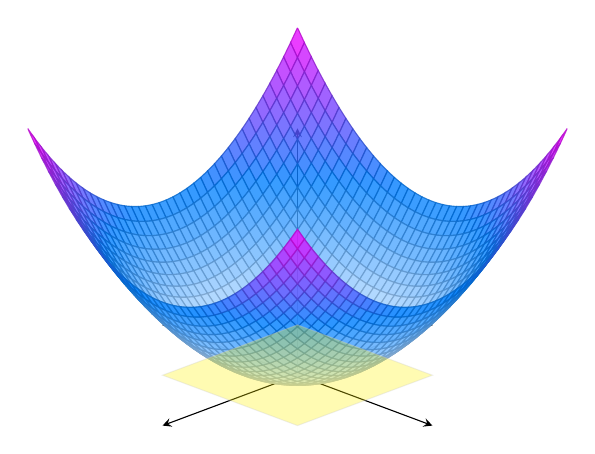
\begin{tikzpicture}
  \begin{axis}[
      view={135}{30},
      colormap/cool,
      axis lines=center,
      xlabel={}, ylabel={}, zlabel={},
      domain=-2:2,
      y domain=-2:2,
      samples=40,
      samples y=40,xtick=\empty,
ytick=\empty,
ztick=\empty
    ]

    % Paraboloid surface z = x^2 + y^2
    \addplot3[
      surf,
      opacity=0.8
    ]
    {x^2 + y^2};

    % Tangent plane at origin z = 0
    \addplot3 [
      surf,
      domain=-1:1,
      y domain=-1:1,
      samples=2,
      samples y=2,
      fill=yellow,
      opacity=0.3
    ]
    {0};

  
   

  \end{axis}
\end{tikzpicture}
    \caption{Notice how all the tangents at the lowest point of the paraboloid $(x=0,y=0)$ is constrained to be in the yellow coloured plane. Now only some area around $x=0,y=0$ can be made to look locally like the yellow plane and hence the definition of velocity will be valid only locally, within that patch.   }
\end{figure}
\subsection{Affine Connection}
